
Nuestra implementaci\'on de la TaskConsola consiste en un ciclo que realiza $n$ (el primer par\'ametro de la tarea) interrupciones. 
Para determinar la cantidad de tiempo que debe durar cada interrupci\'on empleamos la funci\'on $std::rand()$ de la librer\'ia est\'andar. 
Sin embargo, es necesario normalizar el resultado de \'esta, ya que devuelve un valor entre $0$ y $RAND\_MAX$ (un macro definido en $stdlib.h$, dependiente de la implementación) y necesitamos que est\'e entre $bmin$ y $bmax$ (los otros dos par\'ametros de la tarea).

Para lograr esto, dividimos el valor aleatorio inicial por $RAND\_MAX - 0$, para obtener un n\'umero perteneciente al intervalo $[0, 1]$.
Luego, lo multiplicamos por $(bmax - bmin)+1$, obteniendo un resultado perteneciente al conjunto $[0, bmax - bmin + 1]$.
Finalmente sumamos $bmin$ y obtenemos un valor perteneciente al conjunto $[bmin, bmax + 1]$.
Si bien esto puede parecer incorrecto, el cast de un $double$ a un $int$ en C++ toma la parte entera del $double$, por lo que este conjunto es el deseado. 

El \'unico caso donde el resultado puede no llegar a ser el deseado es donde el valor es exactamente $bmax + 1$. 
Si bien esto no puede pasar en una variable continua (como ser\'ia te\'oricamente la uniforme que estamos manejando), al tratar con una representaci\'on de m\'aquina de los reales (como son los $doubles$) esto es posible (y sucede cuando $rand()$ devuelve exactamente $RAND\_MAX$).
Para evitar este error, si el resultado final es exactamente $bmax + 1$, le asignamos $bmax$.

En la figura \ref{fig:figuraEj1} se puede ver un ejemplo de un lote de tareas con dos Task Consolas (ambas con par\'ametros $n = 5$, $bmin = 1$ y $bmax = 3$).

\begin{figure}[H]
\caption{Ejemplo de un lote de tareas con Task Consola}
\label{fig:figuraEj1}
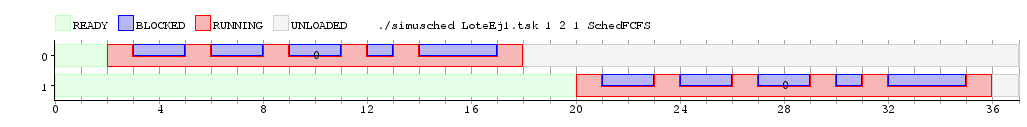
\includegraphics[width=1\textwidth]{imgs/imgEj1.png}
\end{figure}

